% Report --- ks1591
% include a brief discussion about how the limitation of leaf instances affects the performance of the decision tree algorithm.

\documentclass[12pt,a4paper,twocolumn]{article}
\usepackage{times} % times font
\usepackage{mathptmx} % times font in maths
% \usepackage{fullpage}
\usepackage[top=0.55in, bottom=0.7in, left=0.7in, right=0.7in]{geometry}
\usepackage{multirow} %in tables
\usepackage{caption} % in tables
\pagenumbering{gobble}
\newcommand{\HRule}{\rule{\linewidth}{0.5mm}}

\usepackage[pdftex]{graphicx}
\usepackage{lipsum}
\usepackage{amsmath}

% \usepackage{hyperref}
% \usepackage{graphicx}
% \usepackage{subfigure}
% \usepackage{indentfirst} % indent frst paragraph of section

% \usepackage[usenames,dvipsnames]{color}

% \newcommand{\ts}{\textsuperscript}

\begin{document}

\twocolumn[
\begin{@twocolumnfalse}
\begin{center}
	\begin{large}
	{\HRule \\[0.2cm]}
	\textsc{Spiking Integrate and Fire model of neuron}
	{\HRule \\[0.3cm]}
	\end{large}

	\begin{minipage}{ 0.44\textwidth }
		\begin{flushleft}
			Kacper \textbf{Sokol}\\
			\texttt{ks1591} --- 3GGK1
		\end{flushleft}
	\end{minipage}
	\begin{minipage}{ 0.44\textwidth }
		\begin{flushright}
			{COMS30127 $|$ Computational Neuroscience\\
			Lab 1: Simulation of a single neuron\\[0.3cm]}
		\end{flushright}
	\end{minipage}
\end{center}
\end{@twocolumnfalse}
] % \lipsum[1]~\\[0.4cm]

\section*{\texttt{Part 1}}
Simulation of neuron based on \emph{Integrate and Fire} model:
$$ \tau_m \frac{dV}{dt} = E_L - V + R_m I_e $$
with parameters:\\
$\tau_m = 10 \text{ [ms]}$~,~$E_L = V_{reset} = -70 \text{ [mV]}$~,\\
$V_{th} = -40 \text{ [mV]}$~,~$R_m = 10 \text{ [M$\Omega$]}$~,\\
$I_e = 3.1 \text{ [nA]}$~,~$DT = 1 \text{ [ms]}$~.

\begin{figure}[htbp]
\centering
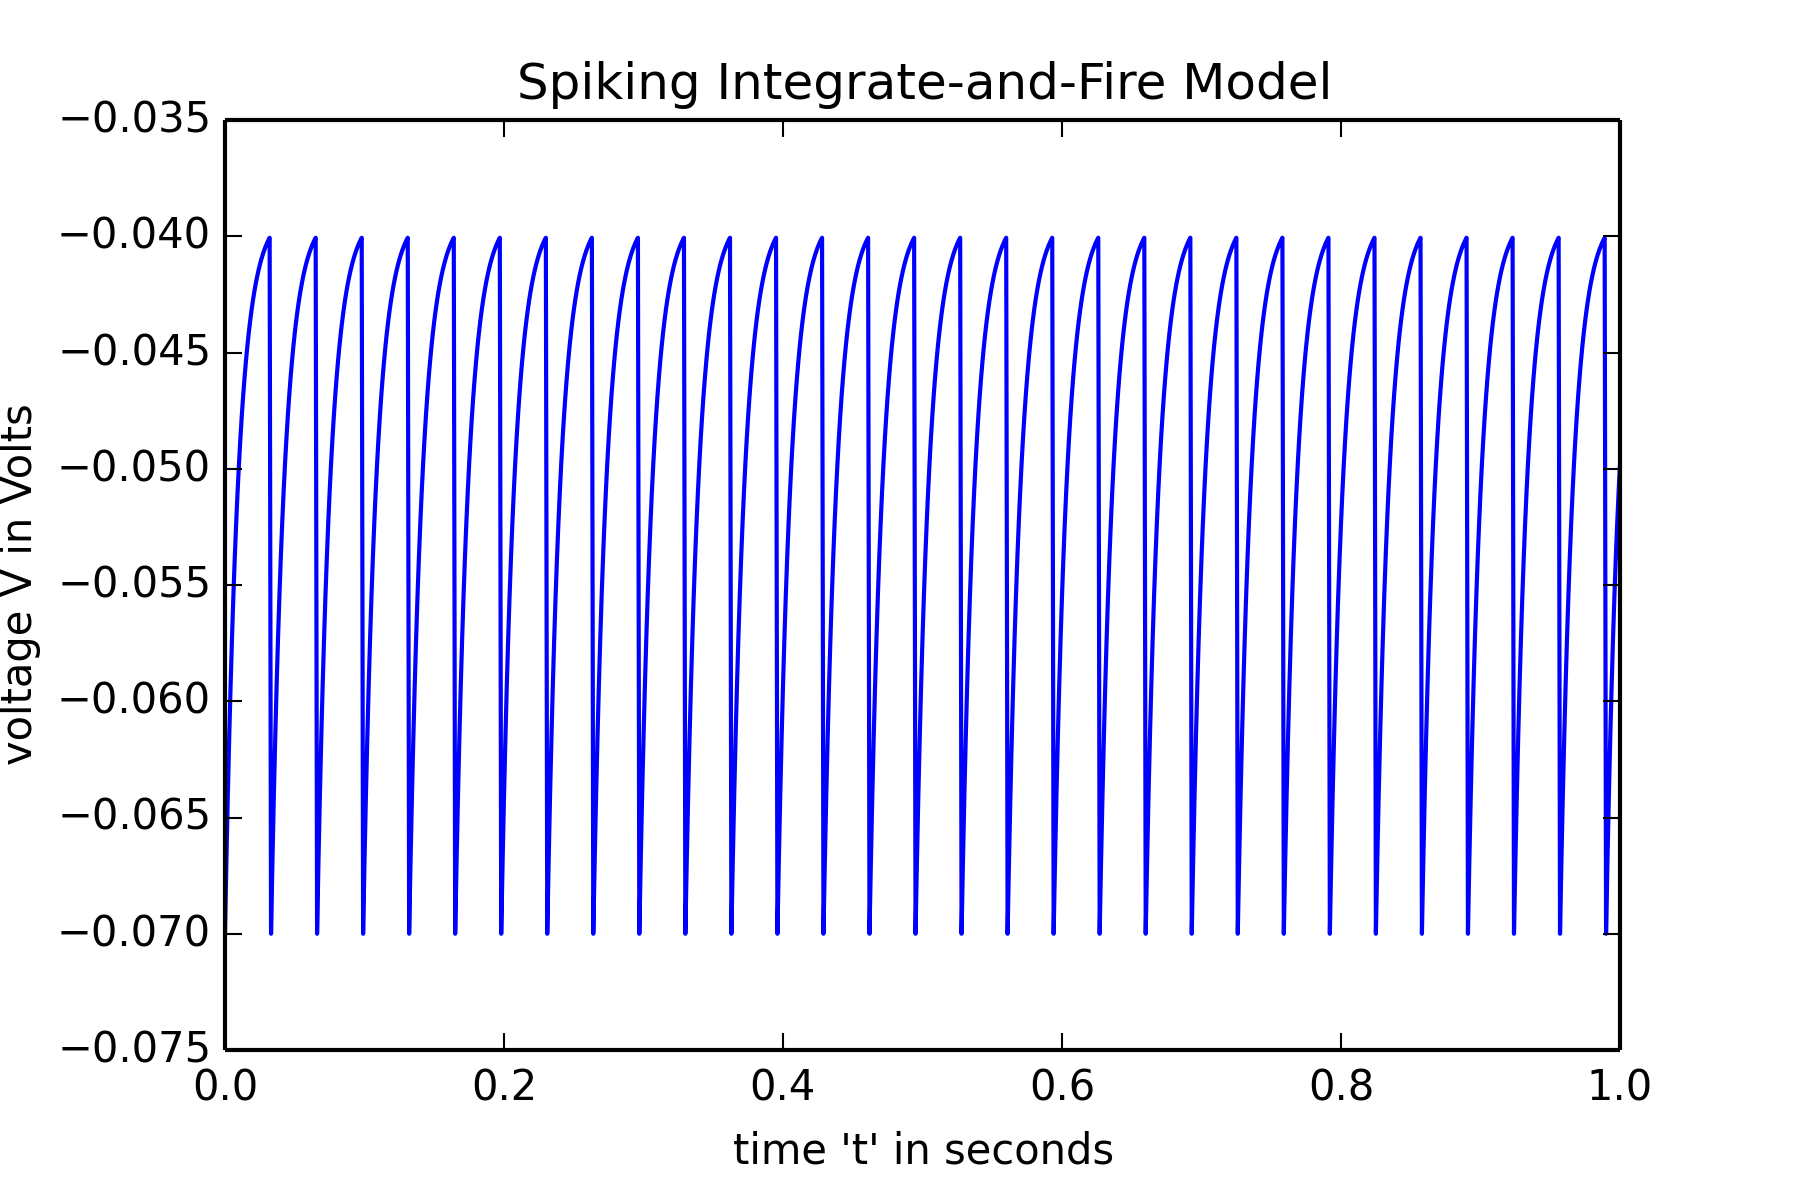
\includegraphics[width=0.5\textwidth]{figures/figure1.png}
% \begin{tiny}
\caption{Simulation of \emph{Spiking Integrate and Fire} neuron model.\label{fig:part1}}
% \end{tiny}
\vspace{0.4cm}
\end{figure}


\section*{\texttt{Part 2}}
\subsection*{\texttt{Part 2: a)}}
\textbf{\large Finding attractor}\\
To analytically compute minimum current $I_e$ required by neuron to produce a spike we set derivative to 0.\\
$0=E_L-V^{\star} +R_mI_e$,\\
$V^{\star} = E_L + R_mI_e$,\\
and we need: $V^{\star} > V_{th}$ for neuron to fire,\\
$E_L+R_mI_e > V_{th}$ hence,\\
$I_e > \frac{V_{th} - E_L}{R_m}$\\
With our parameters:\\
$I_e > \frac{-40*10^{-3} - (-70)*10^{-3}}{10*10^6}$ hence:\\
$I_e > 3 * 10^{-9}$.\\

\subsection*{\texttt{Part 2: b)}}
Simulating neuron with $I_e = 2.9 * 10^{-9}$ leads to behavior shown below.\\

\begin{figure}[htbp]
\centering
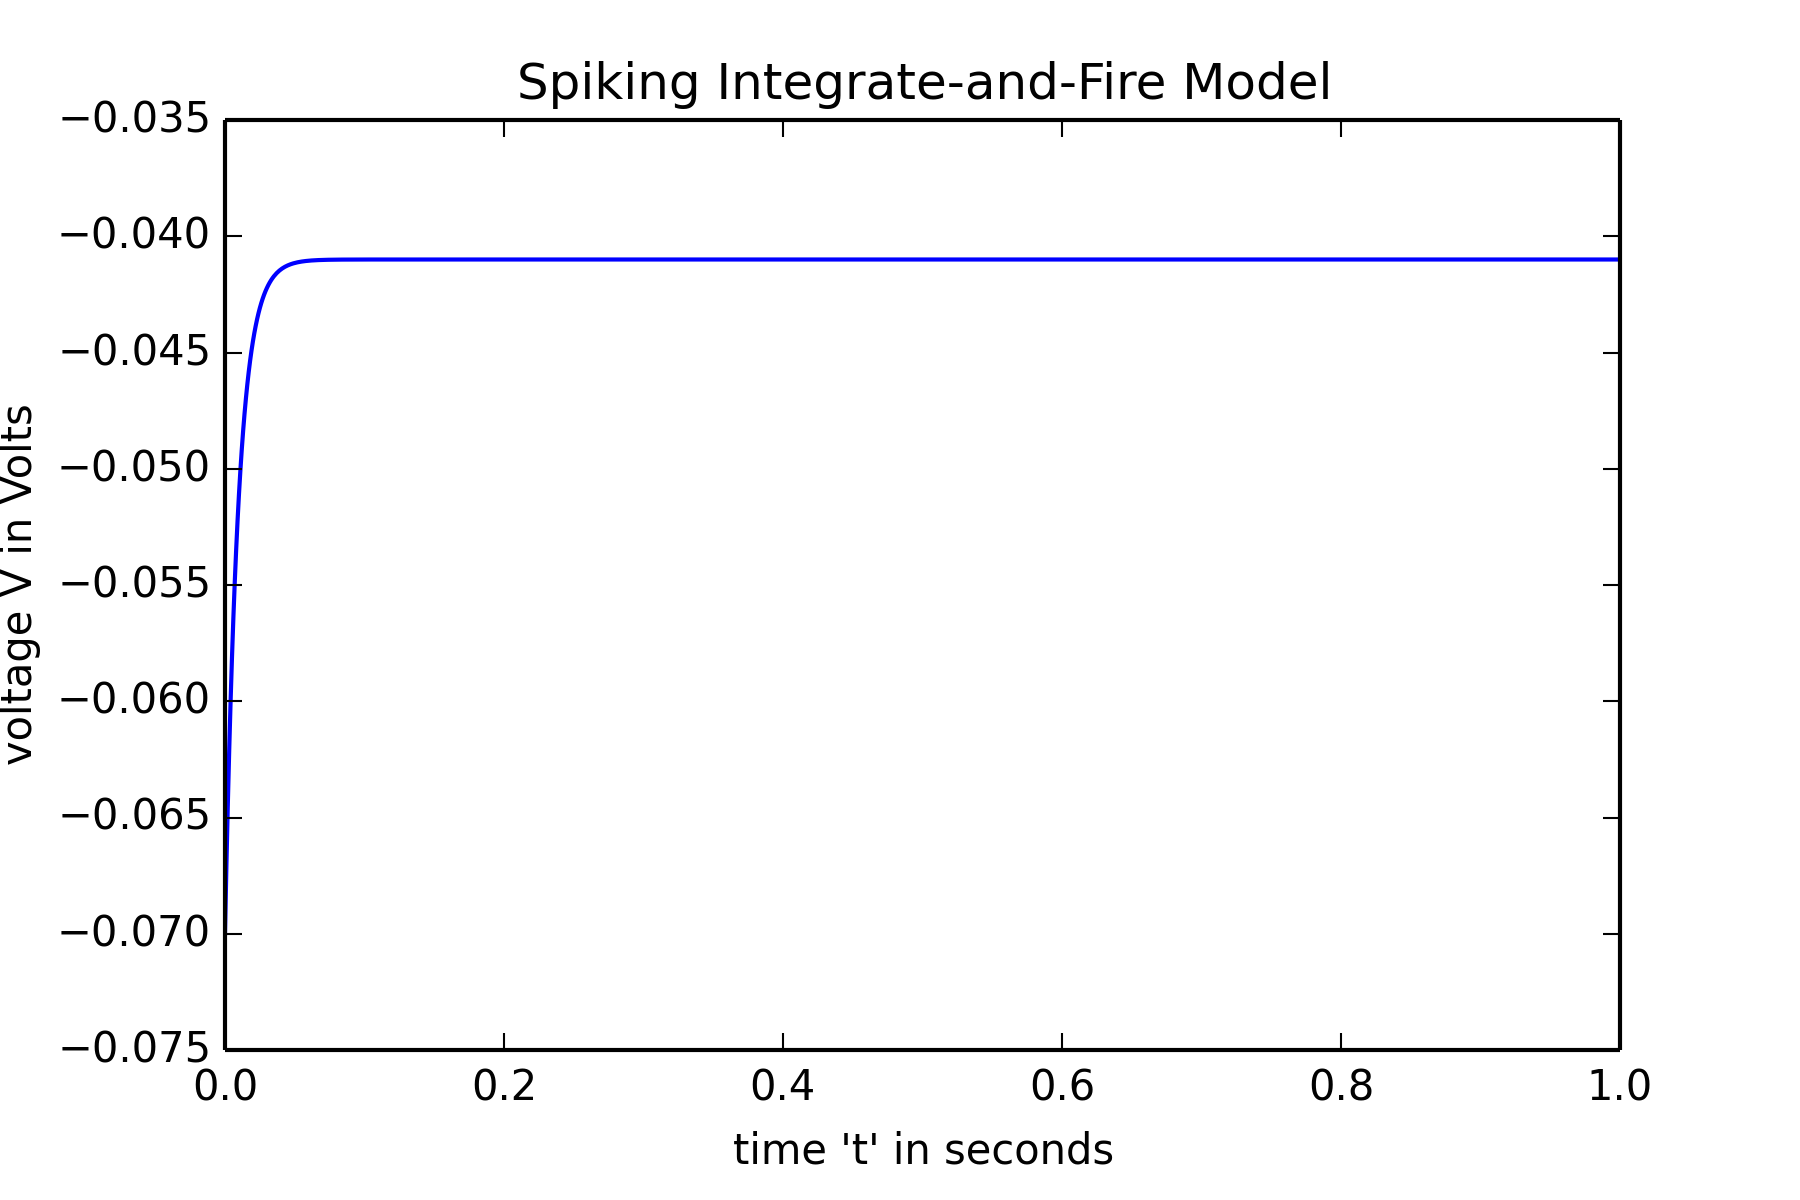
\includegraphics[width=0.5\textwidth]{figures/figure2b.png}
% \begin{tiny}
\caption{Simulation of neuron with current $I_e$ being to small to cause spiking.\label{fig:part2b}}
% \end{tiny}
\vspace{0.4cm}
\end{figure}

\section*{\texttt{Part 3}}
Simulation of neuron for currents ranging from $2 \text{[nA]}$ to $5 \text{[nA]}$ in increments of $0.1 \text{[nA]}$ with count of number of spikes produced for each step.\\
\begin{figure}[htbp]
\centering
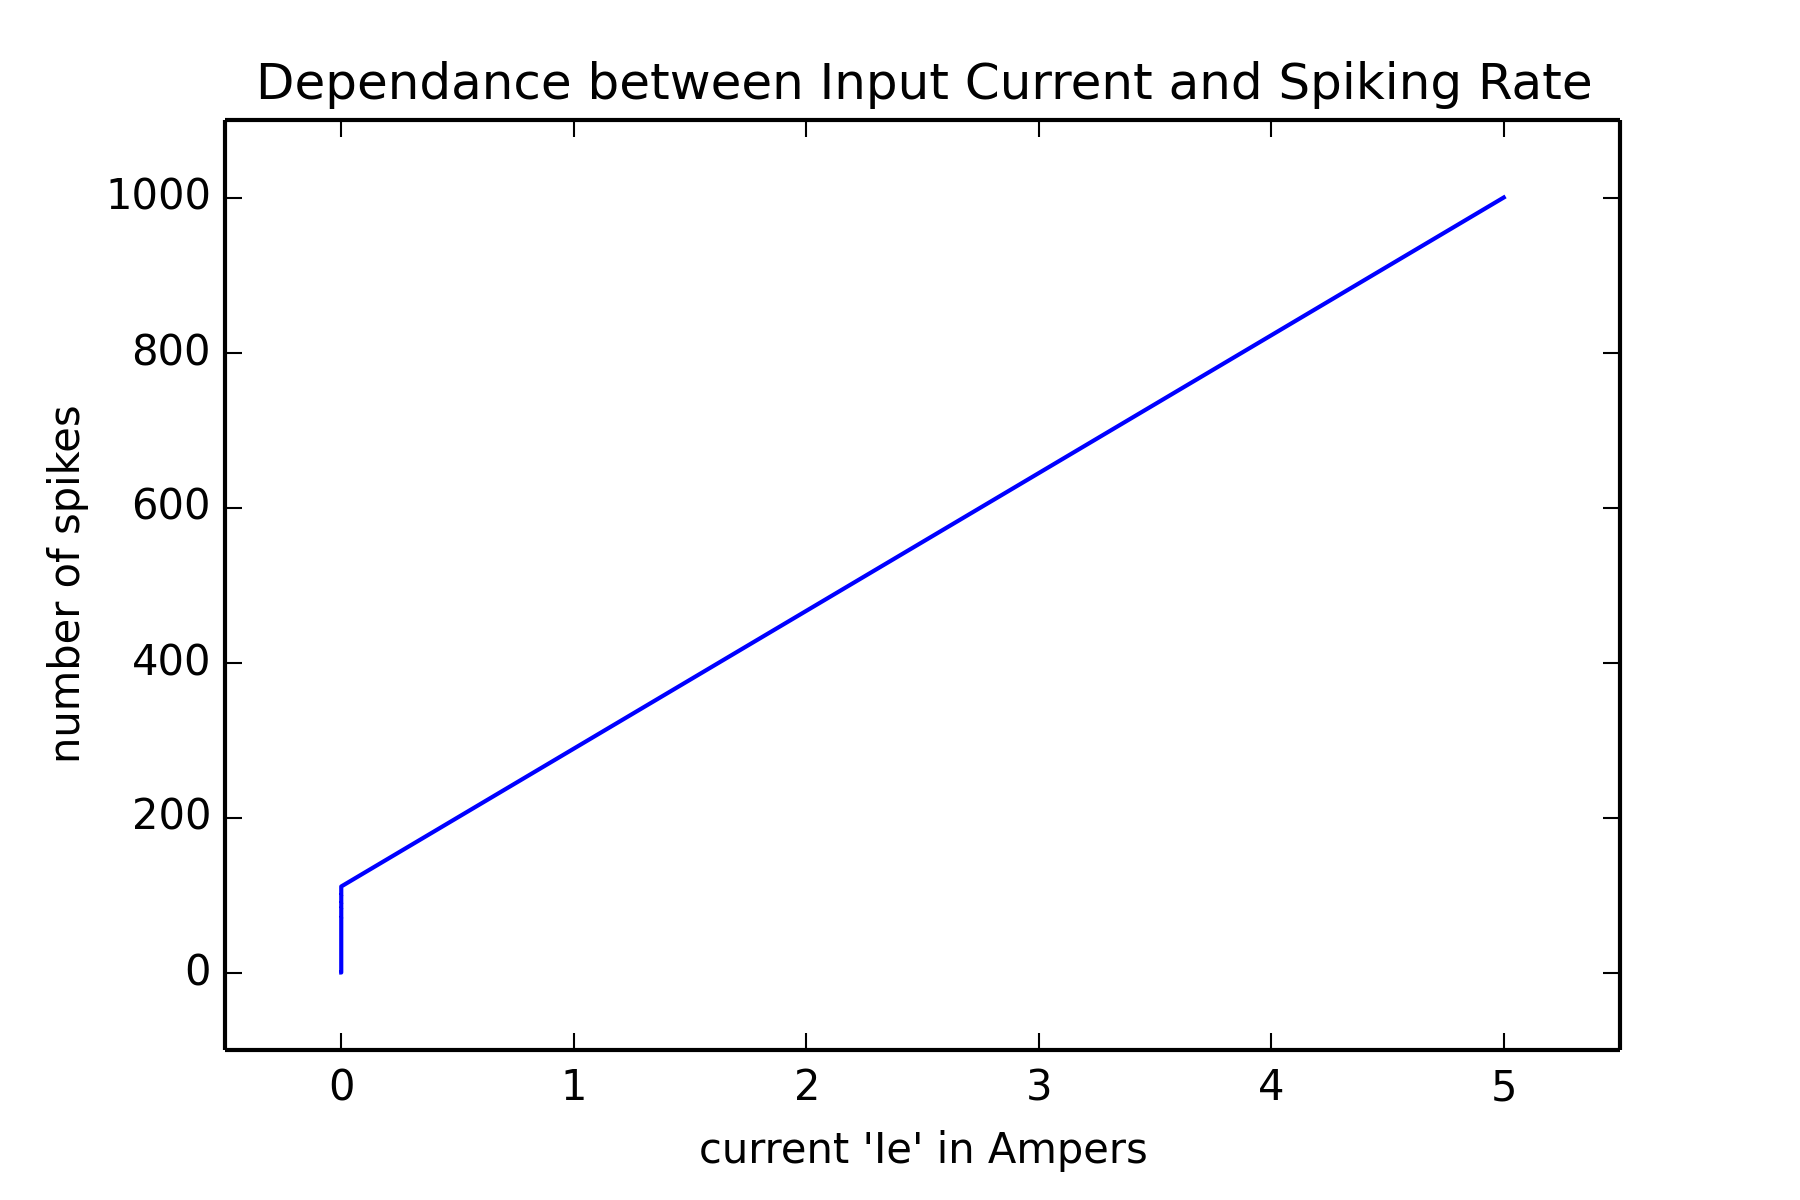
\includegraphics[width=0.5\textwidth]{figures/figure3.png}
% \begin{tiny}
\caption{Firing rate of neuron for given above range of currents.\label{fig:part3}}
% \end{tiny}
\vspace{0.4cm}
\end{figure}

\section*{\texttt{Part 4}}
\textbf{\large Differences between \emph{excitatory} and \emph{inhibitory} synapses}

\subsection*{\texttt{Part 4: a)}}
In first case where synapses are \emph{excitatory} the spikes tend to synchronise. The neuron with excitatory synapse causes other neuron to be more likely to fire at the same time. Both neurons synchronise because they are interconnected so when first one fires it causes that the second one is more likely to fire and the other way around.\\

\begin{figure}[htbp]
\centering
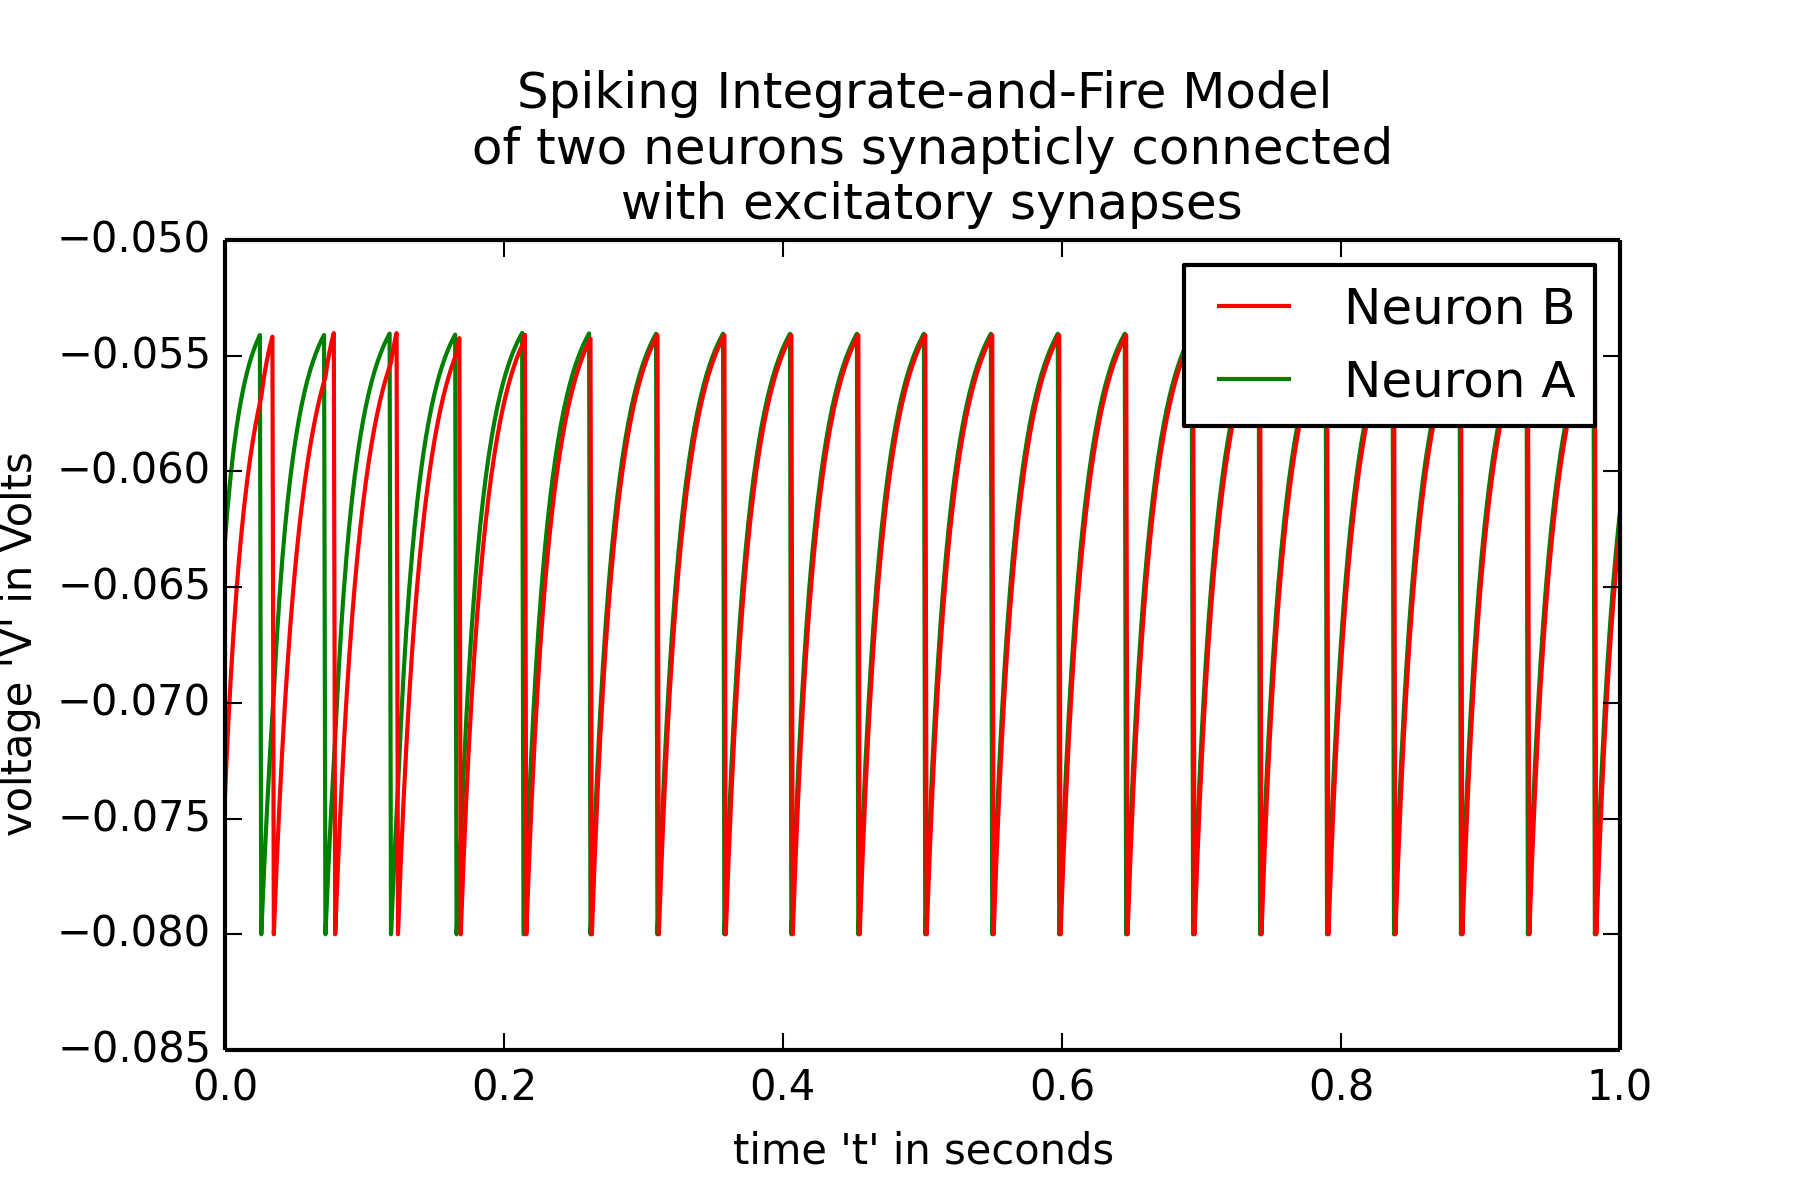
\includegraphics[width=0.5\textwidth]{figures/figure4a.png}
% \begin{tiny}
\caption{Simulation of two interconnected neurons with excitatory synapses.\label{fig:part4a}}
% \end{tiny}
\vspace{0.4cm}
\end{figure}

\subsection*{\texttt{Part 4: b)}}
On contrary, with both synapses being \emph{inhibitory} the spiking tends to diverge. The inhibitory synapse causes connected neuron to be less likely to fire at the same time. Spikes of both neurons diverge as firing of first one causes the second one to be less likely to fire at the same time so at some point the time between firing of one and the other will converge to maximal possible value(spikes maximally distant of each other).

\begin{figure}[htbp]
\centering
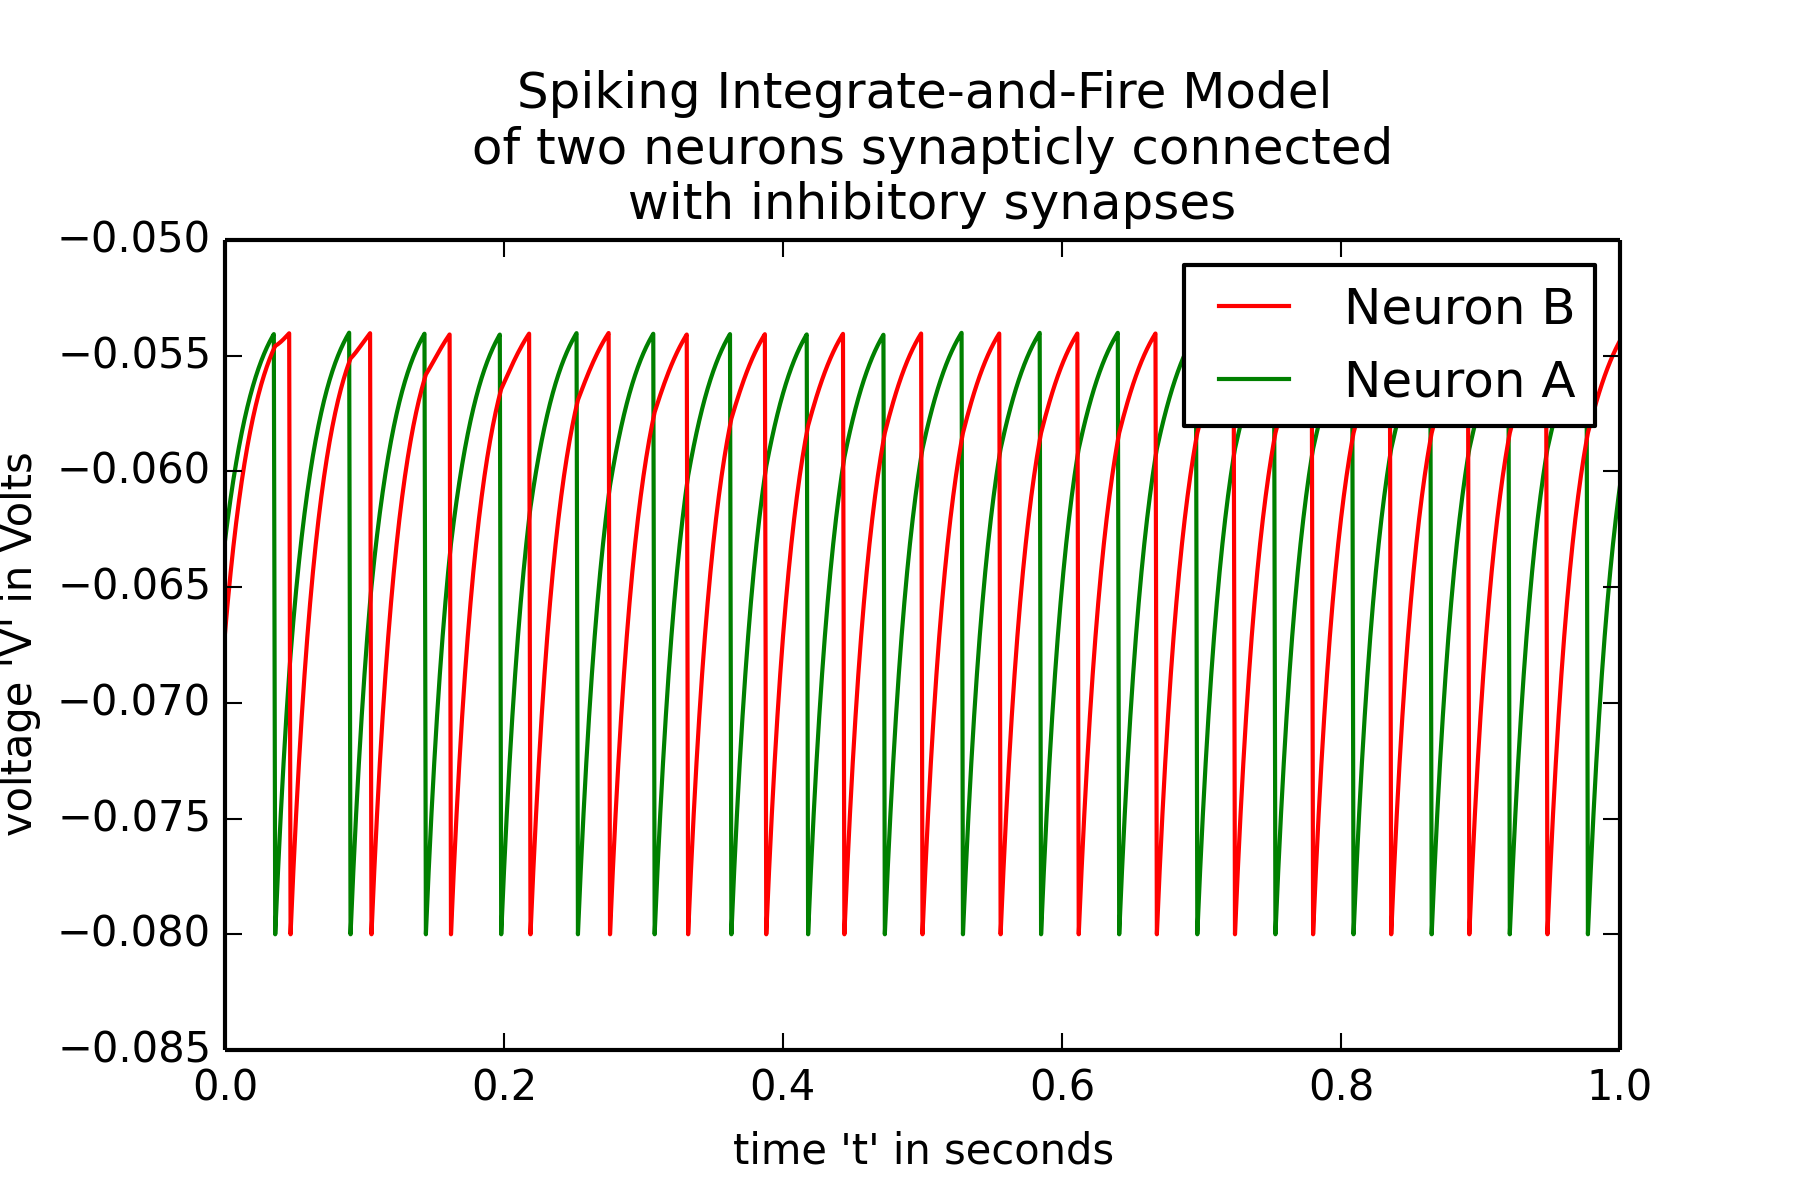
\includegraphics[width=0.5\textwidth]{figures/figure4b.png}
% \begin{tiny}
\caption{Simulation of two interconnected neurons with inhibitory synapses.\label{fig:part4b}}
% \end{tiny}
\vspace{0.4cm}
\end{figure}
\end{document}
